\section{Mémoire}
\commentaire{Idées en cours ainsi que re formulation}


Plusieurs IOT existent sur les voitures et fonctionnent parfaitement sur les motos comme l'angle mort, l'ABS, l'anti-patinage, le contrôle de traction, etc. Cependant, il existe des différences notables entre les deux types de véhicules. Dans cette partie, je vais me consacrer sur l'analyse de la route et l'optimisation des trajectoires.

% faire des schémas avec les trajectoires pour souvelver les problèmes

\subsection{Pratique de la route - Analyse comparative des besoins de sécurité entre voitures et motos}

\commentaire{\\
Analyse des différences fondamentales : protection physique, stabilité, visibilité, comportements routiers.\\
	•	Quelles fonctionnalités IoT des voitures sont difficilement transférables ?\\
•	Quelles fonctionnalités sont transférables mais nécessitent adaptation ?\\
•	Mise en évidence des lacunes spécifiques aux motos.
}


\commentaire{reformulation à faire}
J’ai eu l’occasion d’expérimenter la pratique du deux-roues sous différents angles :\
\begin{itemize}
    \item Les trajets du quotidien,
    \item Les balades entre ami(e)s,
    \item Les road trip de plus d'une dizaine de jours (environ 200 à 300 kms par jour), souvent en milieu montagneux.
\end{itemize}

\vspace{0.5cm}
Avec plus de 35 000 km parcourus en deux ans, voici les constats que j’ai pu faire autour de moi :\\
• Les trajets du quotidien peuvent paraître anodins, mais c’est justement la routine qui les rend dangereux. En connaissant la route par cœur, on a tendance à relâcher sa vigilance, alors que les risques restent bien réels (état de la chaussée, comportement imprévisible des autres usagers, etc.).\\
•	Les balades entre ami(e)s apportent un vrai plaisir de conduite, mais l’effet de groupe peut parfois inciter à dépasser ses limites. On peut se retrouver à rouler à des vitesses inadaptées ou à prendre de mauvaises décisions sous l’influence de comportements plus audacieux. Le jugement individuel peut alors être altéré.\\
•	Les road trips, quant à eux, demandent une grande endurance. La fatigue s’accumule rapidement, et avec elle, le temps de réaction s’allonge. Il est essentiel d’être pleinement en possession de ses capacités pour pouvoir réagir correctement en cas de situation imprévue.\\

Enfin, un point important : lorsque la chaussée est mouillée, la majorité des motards adoptent naturellement une conduite plus prudente, vitesse réduite, prise d’angle limitée, meilleure anticipation. Cela montre que la perception du risque influence fortement le comportement. %transition
Abordons maintenant une difficulté que beaucoup de deux-roues rencontres: les virages.

\vspace{0.5cm}
%TRAJECTOIRES SECURITÉ
\commentaire{idée : montrer que c'est complexe}
Voici des illustrations des trajectoires de sécurité. C'est un thème qui est très abordé par la sécurité routière, les gendarmes ainsi que les usagers des deux-roues. 
\begin{figure}[H]
    \centering
    \includegraphics[width=0.4\textwidth]{coeur_memoire/schéma/trajectoire_sécurité_1.png} 
    \caption{Trajectoire de sécurité utilisée sans obstacle}
\end{figure}
En prenant une trajectoire comme celle-ci, il s'agit ici d'améliorer la visibilité dans le virage. Voici maintenant la trajectoire idéale dès qu'il y a un autre usager sur la route.
\begin{figure}[H]
    \centering
    \includegraphics[width=0.4\textwidth]{coeur_memoire/schéma/trajectoire_sécurité_4.png} 
    \caption{Trajectoire de sécurité utilisée avec un autre usager}
\end{figure}
Instinctivement, le motard va se rapprocher à l'extérieur du virage pour s'éloigner du danger représenté en bleu par la voiture.
Pour poursuivre cette démonstration, nous allons y ajouter d'autres dangers sur la route représentés par des objets en bleu rendant l'impossibilité de prendre une trajectoire "parfaite". Dans la vie courante, cela peut représenter des gravillons, un animal mort sur la route, des plaques d'égout, des nids de poule, des bandes d'étanchéité (mastics), etc. Ces éléments font perdre de suite l'adhérence des pneus et peuvent entraîner une chute. 
\begin{figure}[H]
    \centering
    \includegraphics[width=0.4\textwidth]{coeur_memoire/schéma/trajectoire_sécurité_2.png} 
    \caption{Autre configuration de la route avec plusieurs autres dangers}
\end{figure}
Ajoutons maintenant la trajectoire idéale à la situation permettant de garder l'adhérence des pneus:
\begin{figure}[H]
    \centering
    \includegraphics[width=0.4\textwidth]{coeur_memoire/schéma/trajectoire_sécurité_3.png} 
    \caption{Trajectoire de sécurité utilisée avec des dangers sur la route}
    \label{fig:trajectoire_securite_difficulte}
\end{figure}
Cette trajectoire améliore l’adhérence des pneus, mais elle présente un risque important en cas de danger venant en sens inverse. Si un véhicule surgit en face, le motard dispose de très peu de temps pour réagir ou se décaler, ce qui peut entraîner un accident. Il est donc essentiel d’adapter sa trajectoire en fonction de plusieurs éléments : l’état de la route, la visibilité et la présence d’autres usagers. La vitesse joue également un rôle déterminant : plus la moto roule vite, plus il devient difficile de corriger la trajectoire à temps. Voici ci-dessous plusieurs exemples de trajectoires, chacune présentant ses avantages et ses limites.
\begin{figure}[H]
  \centering
  \begin{subcaptionbox}{Trajectoire possible 1}[0.4\linewidth]
    {\includegraphics[width=\linewidth]{coeur_memoire/schéma/trajectoire_sécurité_7.png}}
  \end{subcaptionbox}
  \hfill
  \begin{subcaptionbox}{Trajectoire possible 2}[0.4\linewidth]
    {\includegraphics[width=\linewidth]{coeur_memoire/schéma/trajectoire_sécurité_6.png}}
  \end{subcaptionbox}
  
  \vspace{0.5cm}
  
  \begin{subcaptionbox}{Trajectoire possible 3}[0.4\linewidth]
    {\includegraphics[width=\linewidth]{coeur_memoire/schéma/trajectoire_sécurité_5.png}}

  \end{subcaptionbox}

  \caption{Autres exemples de trajectoires de sécurité}
\end{figure}

Annalysons et commentons ces trajectoires:\
\begin{itemize}
    \item Trajectoire 1 : C’est la plus sécurisante. Elle permet de s’éloigner efficacement du véhicule venant en sens inverse. Toutefois, si la vitesse est trop élevée, il sera difficile de revenir à l’intérieur du virage, comme le montre la trajectoire en vert.
    \item Trajectoire 2 : Elle est plus risquée, car elle place le motard plus près du danger potentiel. Même si la courbe semble fluide et permet une prise de virage à vitesse plus élevée, elle réduit la marge de manœuvre en cas d’imprévu.
    \item Trajectoire 3 : Elle représente un bon compromis, car elle maintient une certaine distance avec les véhicules en face. Cependant, rester trop proche du bas-côté peut s’avérer dangereux, notamment en cas d’obstacle imprévu (dégradation de la chaussée, présence d’un animal, etc.). La visibilité y est également plus restreinte, ce qui peut compromettre l’anticipation, l'analyse du virage.
\end{itemize}
Pour conclure sur ces schémas, il existe de nombreuses trajectoires possibles, mais peu sont réellement adaptées aux spécificités de la conduite moto. Certaines sont plus risquées que d’autres, et l’expérience du pilote joue un rôle clé dans le choix et la gestion de la trajectoire. Cela met en évidence à quel point cette phase de conduite est exigeante et complexe et combien de facteurs doivent être pris en compte pour envisager une assistance efficace.
%ETUDE SONDAGE
\todo{ajout des réponses d'une enquête partagé sur les réseaux, expériences etc...}
J'ai réalisé une enquête dans différents groupes de motards sur les réseaux sociaux afin de récupérer leur ressenti. L'échantillon est composé d'une petite vingtaine de personnes avec 58,8 \% d'hommes contre 41,2 \% de femmes.
Voici les différents profils des participants :
\begin{figure}[H]
  \centering
  
  \begin{subcaptionbox}{Age des participants}[0.4\linewidth]
    {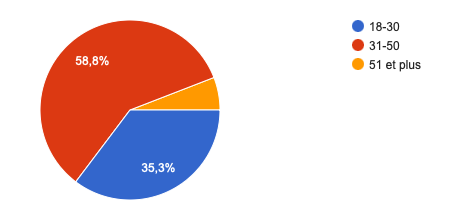
\includegraphics[width=\linewidth]{coeur_memoire/graphique/age.png}}
  \end{subcaptionbox}
  \hfill
  \begin{subcaptionbox}{Nombre d'années de permis}[0.4\linewidth]
    {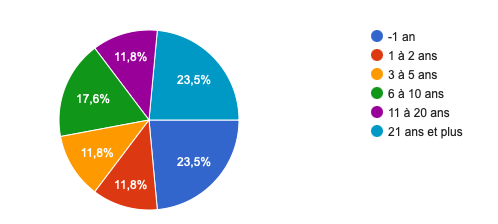
\includegraphics[width=\linewidth]{coeur_memoire/graphique/nb_annees_permis.png}}
  \end{subcaptionbox}

  \begin{subcaptionbox}{Nombre de kms à l'année}[0.4\linewidth]
    {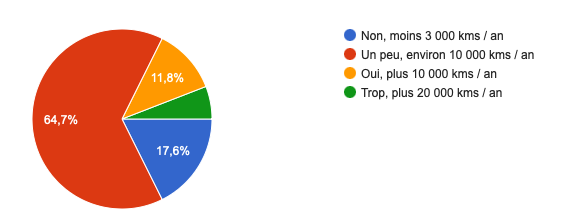
\includegraphics[width=\linewidth]{coeur_memoire/graphique/nb_km_an.png}}
  \end{subcaptionbox}
  \hfill
  \begin{subcaptionbox}{Utilisation de la moto}[0.4\linewidth]
    {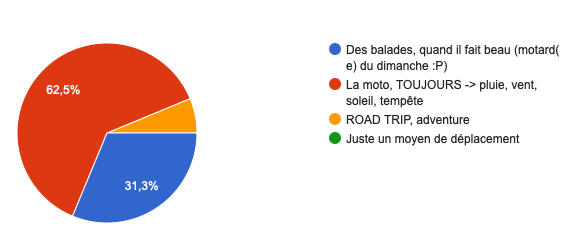
\includegraphics[width=\linewidth]{coeur_memoire/graphique/utilisation_moto.png}}
  \end{subcaptionbox}
  \caption{Profils des participants}
\end{figure}

Pour conclure, lors de cette enquête, il y a tous types de motards. Beaucoup roulent moins de 3 000 kms/an ce qui est très peu. C'est moins d'expérience sur la route.

\todo{ajout bilan des retours de l'enquête}
Lors de mon enquête, la plupart des usagers possèdent des deux-roues roadster comme des 400 cc à 600 cc. On retrouve des Honda, Kawasaki, Aprillia, KTM et Yamaha. Ce sont des motos qui sont inférieures à 10 000 euros.
Pour les voyages, ou bien les voyages dans les Alpes, on aperçoit une majorité de motards qui roulent en GS\footnote{Gelände/Straße : tout-terrain/route. C'est une moto conçue pour être à la fois confortable sur route et capable de rouler sur des chemins non gouderonnés. Premiers prix : 12 000 euros, haut de gamme : environ 30 000 euros.}. On estime entre environ 50 et 70\% des motos rencontrées dans les Alpes (Suisse, Italie et France) sont des GS.\\
Voici quelques retours d'expérience des motards en situation d'urgence selon l'enquête :\\
• "Proche d'un rond-point, j'ai mal évalué la distance. Donc je suis arrivée trop vite, j'étais déjà dans l'insertion sur le rond-point et j'ai failli terminer dans un véhicule. Contrainte d'effectuer un freinage d'urgence et de me mettre le plus à l'extérieur pour éviter la catastrophe."\\
• "La voiture de La Poste stationnée en plein virage en sens inverse, empiétant sur ma voie. Sur une route à 50 km/h en agglomération. J'ai dû pratiquer l'évitement pour ne pas me prendre le véhicule."\\
• "Ma roue s’est coincée dans un rail de tram .. "\\
• "J'ai pris un trou (pas visible avant d'être dedans) sur une nationale, ce qui m'a fait guidonner, impossible à rattraper donc la moto a fini par se coucher et une belle glissade pour finir."\\
• "Évitement de personne qui tourne sans avoir mis de clignotant. Classique."
\vspace{0.5cm}

Pour la fin de l'étude, j'ai demandé aux participants quelles sont leurs attentes concernant les technologies IoT sur les motos. Certains ne souhaitent pas de technologie IoT, car ils estiment que cela peut nuire à la conduite et à la sensation de liberté. D'autres sont favorables à l'intégration de technologies IoT. Par exemple, un assistant virtuel qui indiquerait au pilote les dangers potentiels sur la route (chausée dégradée, virage dangereux, gravillon...). Les autres retours sont des technologies qui sont déjà présentes sur les motos du marché comme l'ABS, le contrôle de traction, l'anti-patinage, etc. Cependant, d'après certains motards, il faut mettre ces éléments de série et non en option comme l'appel d'urgence.

\vspace{0.5cm}


\todo{Ouverture sur la complexité + énonciation des différents vecteurs}

Le défi ici c'est de pouvoir adapter la trajectoire en temps réel, en fonction de la vitesse, de l'angle d'inclinaison, des conditions de la route et des autres usagers. Les technologies IoT peuvent jouer un rôle clé dans cette adaptation en fournissant des données en temps réel sur l'environnement et en permettant une communication entre les différents usagers de la route. La meilleure trajectoire sera celle où le motard se sentira le plus en sécurité. Cela dépend de son expérience, de ses capacités cependant il y a beaucoup de possibilités.


%PLAISIR
\vspace{0.5cm}
Le plaisir de conduire une moto réside dans la sensation de liberté qu'elle procure. Cependant, cette liberté s'accompagne de responsabilités, notamment en matière de sécurité. Les technologies IoT peuvent contribuer à améliorer cette sécurité tout en préservant le plaisir de conduite. "Passionné auto moto depuis mon plus jeune âge, j'aime rouler souvent seul, mais j'aime me sentir libre et pouvoir aller où je veux et quand je veux, la moto, c'est indescriptible et c'est comme une drogue, mais c'est la passion." selon un retour de l'enquête.

\vspace{0.5cm}
Adapter l'IOT représente un défis car il faut prendre en compte de nombreux paramètres (environnement, comportement des usagers, etc.) et s'assurer que les solutions proposées sont adaptées à chaque situation.

\newpage
\subsection{ Étude critique des technologies IoT existantes (voitures vs motos)}
\commentaire{\\
avec un regard critique et des cas concrets.\\
Analyse de cas réels où les technologies IoT ont été adaptées à la moto (Airbags connectés, gilets intelligents, casques IoT, etc.).\\
	Freins techniques : taille réduite, alimentation électrique, exposition météo, vibrations, etc.\\
  lidar et radar ?\\
} \\

%RADAR
La plupart des motos ont les mêmes technologies que les voitures comme l'ABS, la détection d'angle mort, le régulateur adaptatif, ... Et après utilisation, les usagers sont très satisfaits et cette technologie permet de réduire la fatigue et les risques d'accidents.

%LIDAR
\commentaire{reformulation à faire}
Les radars sont utilisés sur les derniers modèles de  motos et ils remplissent très bien leur rôle. Comme évoqué précédemment, les détections de divers choses sur la route sont très importantes pour la sécurité du motard et les actions prises également. Les radars restent très limités. L'utilisation de la technologie lidar est très interessante car elle est douée dans la classification des objets, la cartographie 3D. Cependant, elle  reste très sensible aux conditions météorologiques (pluie, brouillard, neige) et peut être coûteuse (prix, stockage et puissance de calcul) à intégrer sur une moto. De plus, la taille et le poids des capteurs lidar peuvent poser des problèmes de portabilité et d'esthétique sur les motos. Le prix moyen en 2020 d'un LIDAR compacte était entre 3 000 et 10 000 euros selon PW Consulting\cite{marche_capteur_lidar}, ce qui reste très élevé pour un motard. Fort heureusement les prix ont baissé, Aujourd'hui, cette technologie avoisine les 500 - 2000 euros selon les besoins et la gamme.\\
Les prototypes :\\
\begin{table}[ht]
\centering
\begin{tabular}{|l|c|}
  \hline
  Éléments & Prix \\
  \hline
  Capteurs LIDAR & 500 à 2 000 euros \\
  Traitement embarqués & 300 à 1 500 euros \\
  Interfaces et boîtier durci & 100 à 400 euros \\
  Intégration et calibration & 200 à 1 000 euros \\
  Total estimation & 1 100 à 5 900 euros \\
  \hline
\end{tabular}
\caption{Prix moyen estimé pour la technologie LIDAR sur moto (2025)}
\end{table}

Prenons les coûts moyens d'un deux roues :\\
\begin{table}[ht]
\centering
\begin{tabular}{|l|c|c|}
\hline
\textbf{Catégorie} & \textbf{Cylindrée} & \textbf{Prix moyen (TTC, €)} \\
\hline
Scooter & 50--125 cm³ & 2\,000 -- 4\,500 euros \\
Moto légère & 125 cm³ & 3\,500 -- 5\,000 euros \\
Moto moyenne cylindrée & 300--650 cm³ & 6\,000 -- 9\,000 euros \\
Moto grosse cylindrée & 700--1 000+ cm³ & 10\,000 -- 18\,000 euros \\
Moto sportive haut de gamme & 1 000+ cm³ & 18\,000 -- 30\,000 euros \\
Moto électrique & équiv. 50--125 cm³ & 4\,000 -- 12\,000 euros \\
\hline
\multicolumn{2}{|c|}{\textbf{Prix moyen toutes catégories}} & \textbf{7\,000 -- 9\,000 euros} \\
\hline
\end{tabular}
\caption{Prix moyen estimé des deux-roues neufs en 2025 (France/Europe) par The Market Reports}
\end{table}

Pour conclure, la technologie LIDAR peut représenter à elle seule entre 12\% et 84\% du prix d'un deux-roues neuf mais le pourcentage reste moindre pour des voitures haut de gamme avoisinant les 50 000 euros. Cela reste très élevé pour un motard, surtout si l'on considère que la majorité des motards ne changent pas de moto tous les ans. De plus, il faut prendre en compte le coût de l'assurance, de l'entretien, du carburant, etc. Il est donc essentiel de trouver un équilibre entre sécurité et coût pour rendre ces technologies accessibles à tous les motards.

%Autre IOT
Concernant les autres technologies que peuvent proposer les autres marques, elles sont très pertinentes car elles sont destinées pour la sécurité des deux-roues et parfois élaborées par des motards eux-mêmes. Je pense à Géoride par exemple, qui est une application complète.\\
Ce qui peut être intéressant est d'avoir une interopérabilité entre les différents systèmes IoT. Prenons l'exemple de Géoride qui a un système de détection de chute, des motos peuvent l'avoir également ainsi que l'intercom Cardo. Cela permettrait d'éviter trois appels.

\subsection{ Propositions d’adaptations technologiques}
\commentaire{	\\
•	Systèmes de communication V2X (Vehicle-to-Everything) pour motos : miniaturisation, portabilité, est ce que cela est possible ? les conditions.\\
	•	Capteurs embarqués sur la moto et sur le pilote (gilet, casque, smartphone).\\
	•	Intégration d’IA pour la détection du risque en temps réel : freinage d’urgence, angle d’inclinaison, anticipation de collision. => a voir\\
	•	Systèmes d’alerte connectés avec autres usagers (voitures, infrastructures).\\
	•	Possibilité d’un écosystème IoT dédié aux motos, interopérable avec celui des voitures. => à voir si ca existe déja\\
  • modélisation d'un tableau de bord connecté pour moto, avec des capteurs et des alertes en temps réel.\\
}

%PROPOSITION 1 : GPS MOTO 
\todo{parler également de l'accélération}

Pour pouvoir proposer de nouvelles fonctionnalités de prévention, il faut optimiser le tableau de bord. Il faut créer des logos communs à tous pour avoir le même langage. 

\todo{ajout d'un tableau de bord connecté avec des capteurs et des alertes en temps réel.}
L'idée serait d'intégrer dans les motos une puce GPS qui serait capable d'avertir en cas de virage dangeureux. L'alerte (sonore via un intercom et voyant au tableau de bord) serait envoyée via le tableau de bord connecté si la vitesse est supérieure à la vitesse recommandée. Cette vitesse sera calculée via la valeur de la courbure du virage. Des chercheurs Alex Liniger et Simon Hecker ont développé un prototype , Aegis Rider AG\cite{vitesse_virage_mcnews} permettant de prendre la meilleure trajectoire. Cependant, ce dernier ne prend pas en compte les autres facteurs de la route (autres usagers, état de la chaussée, etc.). Comme démontré ci-dessous, la trace bleu indiquant la trajectoire de sécurité et le compteur de vitesse masquent la qualité de la route par conséquent, le motard ne pourra pas anticiper les dangers de la route (gravillon, trous, ....). À l'heure d'aujourd'hui, cette solution reste extrêmement complexe. Ma solution permettra de fonctionner dans la pluspart des cas.

\begin{figure}[h]
    \centering
    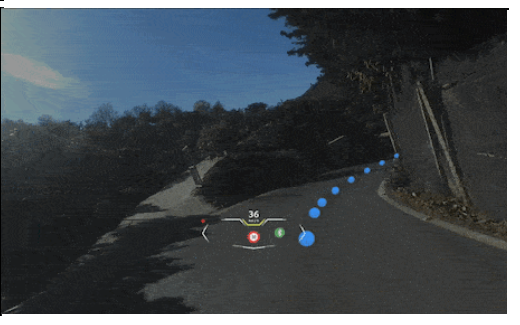
\includegraphics[width=0.7\textwidth]{coeur_memoire/images/aegis.png} 
    \caption{Prototype Aegis Rider AG pour la détection de virages dangereux.}
\end{figure}
Cette fonctionnalité est très interessante mais elle empêche une bonne visibilité de la surface de la route et elle peut fausser une prise de décision.
Comme illustré dans la Figure~\ref{fig:trajectoire_securite_difficulte}, le processus ne pourra pas adapter sur des virages dit "imparfaits".


\todo{voir pour faire une petite ligne de code ?}

\underline{Contexte:} En balade dans le 77, un motard roule sur une départementale. Dans cette situation, il est équipé d'un boitié GPS qui récupère ses coordonnées en temps réel. Il arrive dans une portion de virages limitée à 70 km/h nommée "Les 17 virages", près d'Arbonne-La-Forêt. Cette série de virages est dangeureuse car la route n'est pas bonne, n'est pas large et l'adhérence n'est pas optimale. De plus, il y a un virage dangereux à l'équerre qui surgit au milieu de cette série. La trajectoire de sécurité est fortement recommandé. Par expérience, avoisiner les 70 km/h est déjà bien au vue de la portion qui y est technique.

\begin{figure}[H]
    \centering
    \includegraphics[width=0.7\textwidth]{coeur_memoire/schéma/Capture d’écran 2025-07-24 à 15.45.48.png} 
    \caption{Point GPS des 17 virages.}
\end{figure}

\todo{photo des 17 virages}



Les coordnnées GPS sont : 48.385171, 2.563108.

\todo{mettre le diagramme}
Voici le diagramme d'action de cette fonctionnalité:\\

\begin{figure}[H]
    \centering
    \includegraphics[width=0.8\textwidth]{coeur_memoire/schéma/Capture d’écran 2025-07-24 à 17.48.10.png} 
    \caption{Diagramme d'action du Système de prévention de virages dangereux}
\end{figure}

Pour réaliser un bout de code sur cette fonctionnalité, j'ai décidé d'utiliser ces bibliothèques :\\
• osmnx\cite{osm_doc} : permet d’interroger OSM (OpenStreetMap) et de récupérer des graphes routiers.\\
•	geodesic (de geopy \cite{geopy}) : mesure la distance réelle (en mètres) entre 2 points GPS.\\

L'interêt de calculer la courbure de la courbe est de pouvoir anticiper le virage et par conséquent, adapter la vitesse pour optimiser l'adhérence, la trajectoire où l'on se sentira le plus en sécurité. \\
Le calcul de la courbure permettra d'identifier un virage s'il est dangereux à partir de données GPS cartographiques pour enfin adapter le comportement du système embarqué (alerte, adaptation de trajectoire, assistance..).
Donc la courbure mesure à quel point une route peut changer de direction sur une courte distance, ici, dans un virage.\\
Une route droite a une courbure environ égale à 0. Une route qui tourne fort (virage serré) a une courbure élevée.

\begin{table}[ht]
\centering
\begin{tabular}{|l|c|c|c|}
\hline
Route & Rayon du virage & Courbure (simplifiée) & Risque \\
\hline
ligne droite & infini & 0 & faible \\
Virage large autoroute & 500 m & Faible (0.01) & faible \\
Virage serré en montagne & 30 m & Forte (0.1–0.2) & Élevé \\
\hline
\end{tabular}
\caption{Exemple en pratique}
\end{table}

Un virage serré avec une courbure > 0.1 est souvent dangereux à +60 km/h, surtout à moto.
Plusieurs études indiquent que les rayons < 50 m sont classés comme virages dangereux pour les motos. À plus de 60 km/h, une moto doit pencher à plus de 35°à 40° dans le virage ce qui augmente énormément le risque de chute, surtout s’il y a du gravier, pluie, vent latéral…
L’estimation “courbure > 0.1 = danger > 60 km/h” est une règle empirique, basée sur des données de sécurité moto reonnues, des normes d'ingénierie routière et des approximations géométriques issues de GPS.


L'avantage d'avoir un calcul automatique et en amont, cela permet de prévenir avant même d'être dans le virage. Il peut remplacer un panneau quand celui-ci n'est pas visible. Elle ne remplace pas une analyse dynamique complète mais elle est suffisante pour alerter automatiquement le pilote ce qui est exactement l’objectif du système.



\begin{tcolorbox}[title=Calcul de la courbure]
Courbure mathématique\cite{formule_curvature} d’un virage:
\[
courbure\_virage = \kappa = \frac{1}{R}
\]
où R est le rayon du virage\\
Forme simplifiée de la courbure basée sur la déviation par rapport à une ligne droite.\\
a, b et c sont trois points dans la courbe.\\
\[
curvature = abs((a + b - c) / (a + b))
\]
a + b = distance réelle parcourue en suivant la route \\
c = distance directe entre le début et la fin (comme si on traçait une corde)
\end{tcolorbox}

\begin{figure}[H]
    \centering
    \includegraphics[width=0.7\textwidth]{coeur_memoire/schéma/Capture d’écran 2025-07-22 à 16.27.35.png} 
    \caption{Schéma présentant une moto avant un virage}
\end{figure}


\todo{illustration, développement}

\todo{Détailler le code}

\lstinputlisting[language=Python]{coeur_memoire/programme1.py}


\todo{résultat}
Suite de la mise en situation réelle. Les passages étudiés ont été réalisé bien avant l'expérience, par conséquent, il n'y a aucune notion de vitesse. Chaques passages ont été faits sur la capacité au moment t de l'usager. Voici un premier passage à 51 km/h.
\begin{figure}[H]
    \centering
    \includegraphics[width=0.6\textwidth]{coeur_memoire/images/Capture d’écran 2025-07-28 à 15.56.58.png} 
    \caption{Premier passage dans Les 17 virages}
\end{figure}

Résultat du premier passage avec le programme :
\begin{figure}[H]
    \centering
    \includegraphics[width=0.6\textwidth]{coeur_memoire/images/Capture d’écran 2025-07-28 à 16.23.05.png} 
    \caption{Premier passage dans Les 17 virages}
\end{figure}

Voici maintenant un second passage réalisé un peu plus vite.
\begin{figure}[H]
    \centering
    \includegraphics[width=0.6\textwidth]{coeur_memoire/images/Capture d’écran 2025-07-28 à 16.35.23.png} 
    \caption{Deuxième passage dans Les 17 virages}
\end{figure}


\begin{figure}[H]
    \centering
    \includegraphics[width=0.6\textwidth]{coeur_memoire/images/Capture d’écran 2025-07-24 à 16.20.18.png} 
    \caption{Deuxième passage dans Les 17 virages}
\end{figure}

Le deuxième passage est réalisé plus rapidemment (sans excès de vitesse), cependant, la vitesse est trop "rapide" et nécessite de meilleures capacités pour le passer. Il faut que le motard soit à un niveau bien intermédiaire. Comme l'objectif du programme est de faire de la prévention, j'ai décidé de baser sur un niveau de débutant. Pour conclure, il y a un message qui apparaît.

L'idée maintenant est de prévenir l'usager d'un logo universel. Évidemment, la disposition sera optimisée pour chaque écran. Nous pouvons également y ajouter un bip sonore, cela évitera de fixer en permanance le tableau de bord.
\begin{figure}[H]
    \centering
    \includegraphics[width=0.6\textwidth]{coeur_memoire/images/Capture d’écran 2025-07-25 à 14.42.42.png} 
    \caption{Génération d'un tableau de bord possible avec l'IA.}
\end{figure}






\subsection{ Étude de faisabilité et limites}
\commentaire{\\
    •	Quels obstacles (coût, poids, énergie, connectivité, acceptabilité des motards) à l’implémentation ?\\
	•	Quelles pistes pour la recherche ou le développement industriel ?\\
	•	(une maquette fonctionnelle, un prototype conceptuel, ou même une étude de cas simulée)\\
  •	ouverture défi environnemental\\
  •	 protection des données sensibles (lien via kappa)        }

Les limites actuellement restent les prix. En effet, ajouter des fonctionnalités de sécurité ayant des prix trop important baissent l'attractivité des motos. 

\subsection{Apport personnel et positionnement}
\commentaire{\\
	•	proposer qqch de nouveau ou différemment par rapport à l’existant.\\
•	Une vision d’ensemble : comment la réflexion contribue à combler le fossé technologique entre sécurité voiture vs moto.
}

Je pense que la sécurité n'a pas de prix. Que le progrès ne cesse d'évoluer et que dans quelques années, la technologie saura répondre à tous les besoins. La mentalité évolue et il est important d'accompagner cette évolution pour garantir la sécurité des motards. Cela passera par de la sensibilisation, de l'éducation et des technologies adaptées. Je pense que les motards sont prêts à accepter ces changements, à condition qu'ils soient justifiés et apportent une réelle valeur ajoutée à leur expérience de conduite.